\section{Análise da Correlação entre as Taxas de Upload e Download para os Horários com o Maior Valor de Tráfego}

Nesta seção, foi analisada a relação entre as taxas de upload e download para os horários de maior tráfego identificados previamente. Para isso, foram calculados os coeficientes de correlação amostral e gerados gráficos de dispersão (\textit{scatter plots}) comparando as taxas de upload e download para os dispositivos Smart TV e Chromecast.

\subsection{Cálculo do Coeficiente de Correlação}

O coeficiente de correlação amostral foi calculado para cada dispositivo, considerando os datasets correspondentes aos horários selecionados:
\begin{itemize}
    \item \textbf{Smart TV:} Comparação entre o Dataset 1 (Upload) e o Dataset 2 (Download).
    \item \textbf{Chromecast:} Comparação entre o Dataset 3 (Upload) e o Dataset 4 (Download).
\end{itemize}

Os valores dos coeficientes de correlação para cada dispositivo são apresentados na Tabela~\ref{tab:coeficientes_correlacao}.

\begin{table}[H]
    \centering
    \caption{Coeficientes de correlação amostral entre as taxas de upload e download.}
    \label{tab:coeficientes_correlacao}
    \begin{tabular}{|c|c|}
        \hline
        \textbf{Dispositivo} & \textbf{Coeficiente de Correlação} \\ \hline
        Smart TV & 0.9156 \\ \hline
        Chromecast & 0.0050 \\ \hline
    \end{tabular}
\end{table}

Os coeficientes indicam uma correlação positiva moderada para ambos os dispositivos, sendo ligeiramente mais forte na Smart TV.

\subsection{Gráficos de Dispersão}

Os gráficos de dispersão foram gerados para ilustrar a relação entre as taxas de upload e download para os dois dispositivos. Esses gráficos estão apresentados na Figura~\ref{fig:scatter_plot}.

\begin{figure}[H]
    \centering
    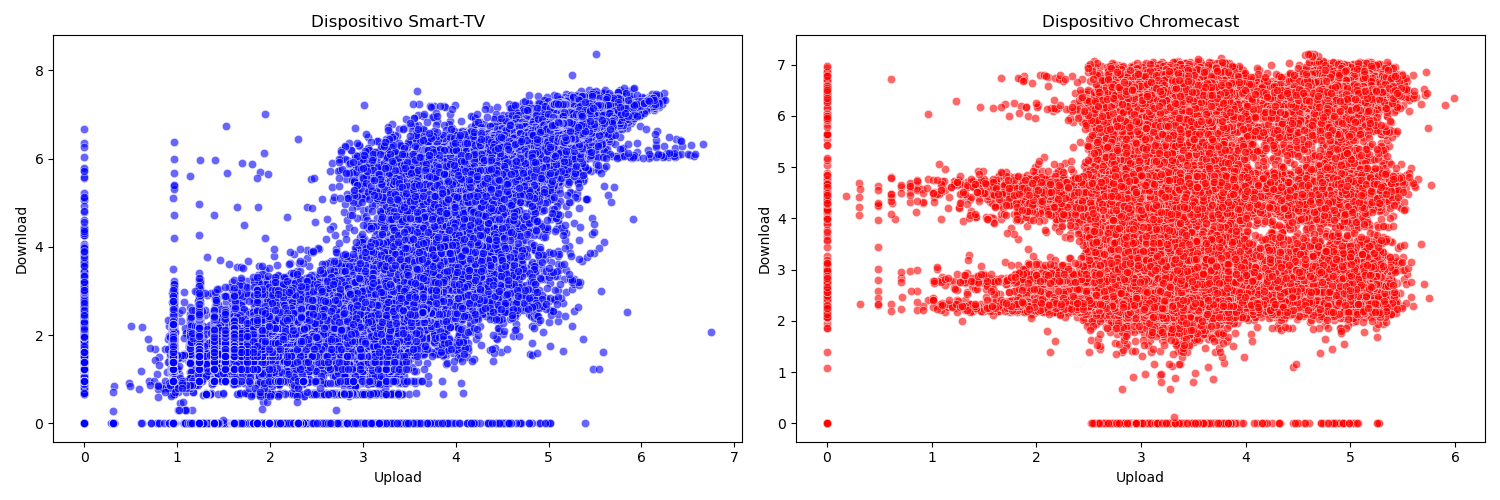
\includegraphics[width=0.8\textwidth]{../correlação/scatter_plot.png}
    \caption{Gráficos de dispersão entre as taxas de upload e download para os dispositivos Smart TV e Chromecast.}
    \label{fig:scatter_plot}
\end{figure}

\subsection{Análise dos Resultados}

Os resultados revelam uma correlação positiva entre as taxas de upload e download para ambos os dispositivos. Para a Smart TV, a correlação mais forte pode ser atribuída a um padrão de uso onde upload e download ocorrem de forma sincronizada, como em transmissões de streaming que requerem alta interação entre o dispositivo e a rede.

Já para o Chromecast, a correlação moderada sugere que as taxas de upload e download possuem menor sincronismo, possivelmente devido a diferenças nos padrões de uso, como bufferizações mais frequentes ou uso em aplicativos de menor interação com a rede.

Essas informações podem auxiliar o provedor de serviços de Internet a identificar padrões de tráfego específicos para cada dispositivo, contribuindo para o planejamento de políticas de qualidade de serviço e alocação de recursos de rede.
